\section{CONCEPTUAL MODEL}

\subsection{Problem Definition}
\href{http://www.neuromedica.com.co/}{Neurom\'edica} is a health services institution (IPS for its abbreviation in spanish), specialized in health care for adult population focused on neurological disorders; this is a specialized center for Grupo \href{https://www.epssura.com/}{SURA}. Their Almacentro complex is in charge of the distribution of medicine for their patients. Recently, they started receiving patients from DEMPOS (another medicine supplier in Colombia) and they are worried about the significant increase in the waiting time of their costumers.

In this complex, patients arrive and take a turn accordingly to their service type and priority, then they enter a queue until they are called into a specific counter; generally, they are called once and the medicine is provided instantly, but sometimes they are recalled a second time. In total, there are 15 counters. Each operator has some service types assigned with certain priorities, but they can also call patients outside these rules. It is important to remark that a patient enters the system exactly when he takes the turn.

In Figure \ref{fig:act_cycl}, the general activity scheme is presented; it depicts the flow of a patient throughout the system; and in Figure \ref{fig:system} we present a minimalist representation of the system at hand.
\begin{figure}[H]
    \centering
    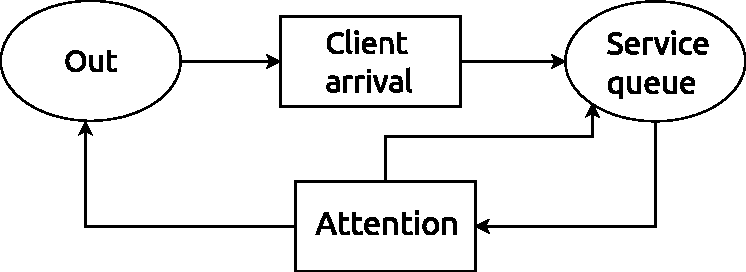
\includegraphics[scale=.8]{files/activity_cycle.pdf}
    \caption{Activity Cycle Diagram}
    \label{fig:act_cycl}
\end{figure}
\begin{figure}[H]
    \centering
    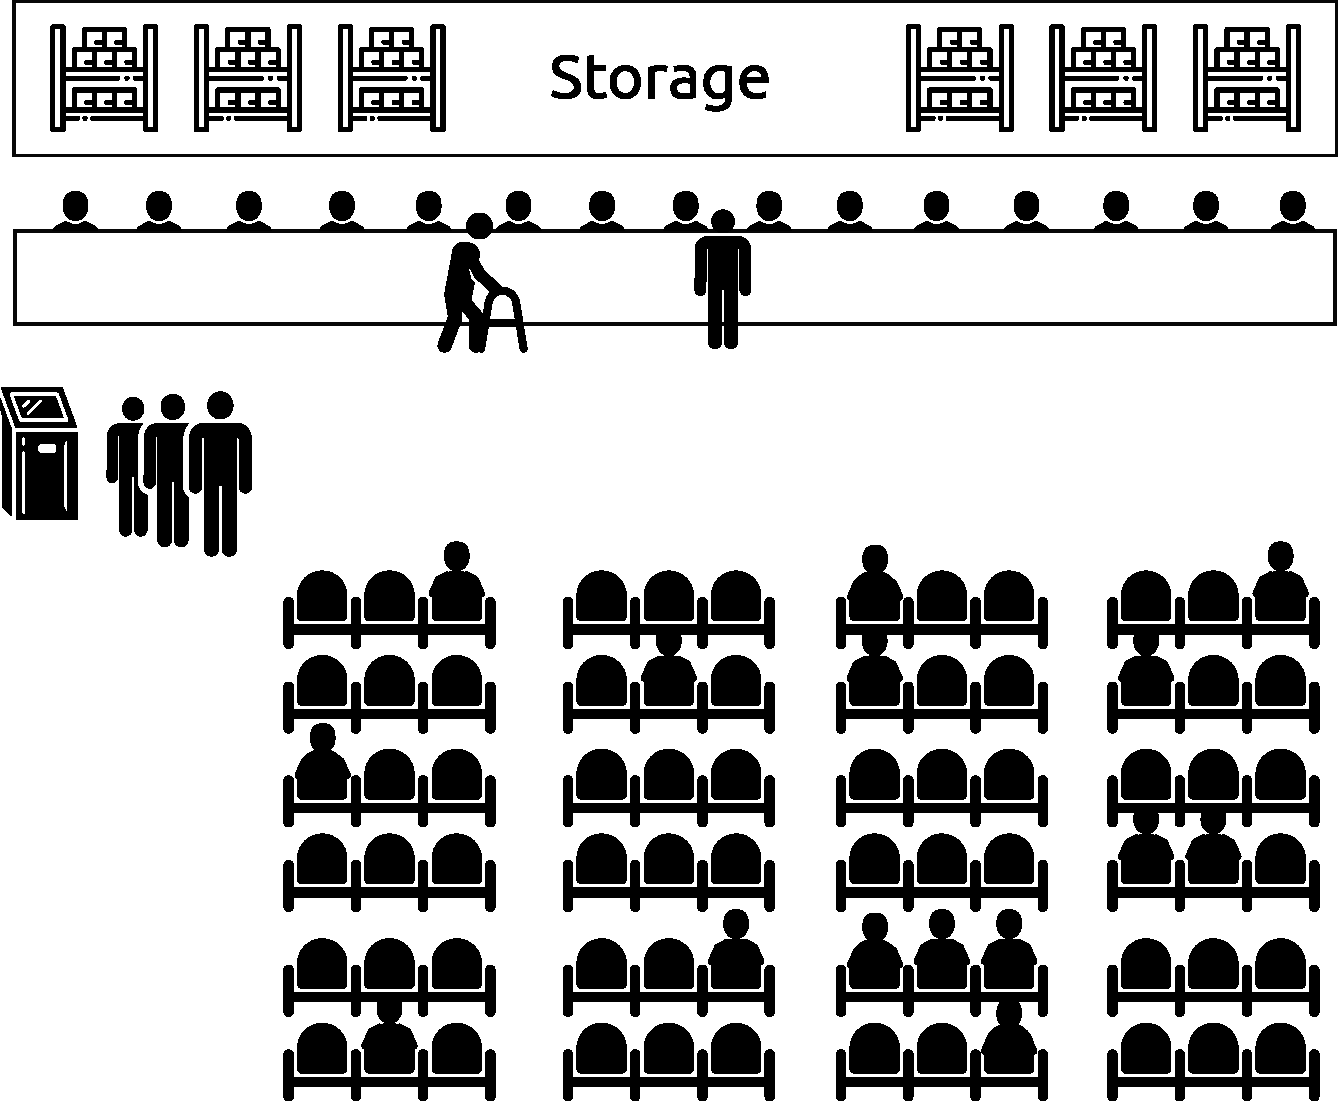
\includegraphics[scale=.5]{files/drawing.pdf}
    \caption{System diagram.}
    \label{fig:system}
\end{figure}

The complex attends the services presented in Table \ref{tab:types_serv}, each service has associated an ID; on the other hand, each module attends specific IDs with certain priorities, as shown in Table \ref{tab:pol_mod}. For example, ``Admissions 1'' attends, first, service 4 which represents ``Appointment confirmation \& PAC, MP and policy SURA''; then it attends service 5 ``Procedure after appointment''; and finally, it calls service 9 ``Preferential appointment confirmation''. It is important to mention that each module can attend outside this policies, for instance, if there are not patients waiting in line with ID 4, 5 or 9, ``Admissions 1'' can call patients with other IDs. Moreover, the attendants can voluntarily call, at any moment, any patient waiting in line.


{\renewcommand{\arraystretch}{1}
\begin{table}[H]
\centering
\begin{tabular}{ll}
\hline
\textbf{ID} & \textbf{Name}                                       \\ \hline
3           & General Pharmacy                                    \\
4           & Appointment confirmation \& PAC, MP and policy SURA \\
5           & Procedure after appointment                                             \\
7           & Preferential Pharmacy                               \\
8           & Pharmacy PAC, MP y SURA policy                      \\
9           & Preferential Appointment confirmation 
         \\
10       & Scheduled retrieval    
\\ \hline
\end{tabular}
\caption{Types of services}
\label{tab:types_serv}
\end{table}

\begin{table}[H]
\centering
\begin{tabular}{ll}
\hline
\textbf{Module}    & \textbf{IDs} \\ \hline
Admissions 1       & 4,5,9        \\
Admissions 2       & 4,9,5        \\
Pharmacy 1         & 3,7,8,10     \\
Pharmacy 2         & 3,8,7,10     \\
Pharmacy 3         & 7,3,8        \\
Pharmacy 4         & 7,3,8        \\
Pharmacy 5         & 3,7,8,10     \\
Pharmacy 6         & 3,8,7,10     \\
Pharmacy 7         & 3,7,8,10     \\
Pharmacy Retrieval & 10           \\
Pharmacy 9         & 3,8,7,10     \\
Pharmacy 10        & 3,7,8,10     \\
Pharmacy 11        & 3,7,8,10     \\
Pharmacy 12        & 3,7,8,10     \\
Pharmacy 13        & 3,8,7,10     \\
Pharmacy 14        & 3,7,8,10     \\\hline
\end{tabular}
\caption{Policy for each module}
\label{tab:pol_mod}
\end{table}
}

\subsection{Modelling Objectives}
\subsubsection{Model Purpose}
To determine the priorities of each module in order to reduce the queue time of patients.
\subsubsection{Specific Objectives}
    \begin{itemize}
        \item To select the most appropriate data to be considered in the model.
        \item To apply statistical tests  to filtered data in order to contrast different hypothesis.
        \item To validate and verify the implemented model using the available data.
        \item To explore multiple feasible strategies for queue priorities in the modules.
    \end{itemize}

\subsubsection{General Project Objectives}
\begin{itemize}
    \item \textit{Time-Scale}: a final report must be available in 5 weeks.
    \item \textit{Flexibility}: high, since our implementation in Python allows us to make modifications easily.
    \item \textit{Ease-of-use}: no, due to its implementation in Python.
\end{itemize}

We decided to implement the model in Python since it allows us to develop a more realistic model, fitting the available data to a wider set of distributions and obtaining a better fit. On the other hand, the Python model is more adaptative for our further experimentation and optimization; although, this kind of implementation makes the model not usable by everyone. Moreover, Python is open-source.

\subsection{Model Inputs \& Outputs}
\subsubsection{Experimental Factors/Model Inputs}
\begin{itemize}
\item Number of modules with priority by hours.
\item Queue logistics.
\item Type of service.
\end{itemize}

\subsubsection{Outputs}
\textit{To determine achievement of objectives:}
\begin{itemize}
    \item Waiting time for each type of patient.
    \item Average time in system.
    \item  Reduce the percentage of patients waiting.
\end{itemize}


\textit{To determine reasons for failure to meet objectives:}
\begin{itemize}
    \item Average number of patients waiting by service type per hour.
    \item  Percentage of people waiting is not reduce.
    \item Leisure time.
\end{itemize}

\subsubsection{Parameters}
\begin{itemize}
\item Inter-arrival times for each type of patient and hour of the day and day of the week.
\item Duration of the attention by type of service and attendant.
\item Probability of quitting.
\item Type of services.
\item Inter-service times for each attendant.
\end{itemize}

\subsection{Model Content}
\subsubsection{Model Scope}
\begin{table}[H]
\centering
\begin{tabular}{p{3cm}lp{6cm}}
\hline
\textbf{Component}                                  & \textbf{Include/Exclude} & \textbf{Justification}\\ \hline
\textbf{Entities:}&&
\\
Customer of each type                      & Include         & This entity is the main character of the simulation.                                                                                                                                             \\
Attendants                                 & Include         & This entity is the one that interact with the costumers and its behavior determines the waiting time.                                                                                           \\
Medicine retrieval attendants & Exclude         & The modelling and simulation of this work assumes that these personnel is always available and the dispatch process is out of the scope of this work. \\
Medicine \mbox{authorization} attendants          & Exclude         & Just as the previous entity, the medicine authorization process is out of the scope of this work.                                                                                                \\\hline
\textbf{Activities:}&&\\
Medicine retrieval     & Include         & This is the activity that each customer is going to be involved. \\
Medicine \mbox{authorization} & Exclude         & There is no way two merge both systems.                          \\ \hline

\textbf{Queues:}&&\\

Dispatch queue      & Include         & Jointly with the last queue, is the focus of this work. \\
Authorization queue & Exclude         & Separate system.                                        \\
Parking lot queue   & Exclude         & Separate system.                                        \\
Delivery services   & Exclude         & Separate system.                                        \\ \hline
\textbf{Resources:}\\
Attendants for \mbox{dispatch} & Exclude         & Number of people that dispatch the medicine.       \\
Medicine               & Exclude         & We assume that there is always available medicine. \\ \hline
\end{tabular}
\caption{Model scope.}
\label{tab:model_scope}
\end{table}

\subsubsection{Model Level of Detail}
\begin{table}[H]
\centering
\begin{tabular}{p{2cm}p{3cm}lp{6cm}}
\textbf{Component}               & \textbf{Detail}                                              & \textbf{Include/Exclude} & \textbf{Justification}                                                                                                                                                             \\ \hline
\textbf{Entities:}               &                                                              &                          &                                                                                                                                                                           \\
Customer of each type            & Customer inter-arrival time varying by hours of the day.     & Include                  & The system at hand clearly has different arrival times for each hour on a day, allowing us to make a more realistic simulation.                                           \\
                                 & Customer inter-arrival time varying by days of the week.     & Include                  & It is important to focus on the busiest days in order to make a more relevant study. It is important to focus on the busiest days in order to make a more relevant study. \\
                                 & Customer inter-arrival time varying by minutes on each hour. & Exclude                  & We believe that considering the inter-arrival time by hours is enough for making significant simulation. Modelling the system by minutes is considered unmanageable.      \\ \hline
\textbf{Activities:}             &                                                              &                          &                                                                                                                                                                           \\
Medicine Dispatch                & Medicine dispatch duration                                   & Include                  & It has a big impact on the waiting time of the customers.                                                                                                                 \\
                                 & Cost per working hours of this attendants                    & Exclude                  & The company did not provide this information and it's not relevant for this work.                                                                                         \\ \hline
\textbf{Queues:}                 &                                                              &                          &                                                                                                                                                                           \\
Authorization and dispatch queue & Customer desertion                                           & Include                  & Modelled as a constant probability. It is important since this clears a spot in the queue.                                                                                \\
                                 & Different types of queues for each type of customers         & Include                  & It is a feasible factor to control.                                                                                                                                       \\
                                 & Queue maximum capacity                                       & Include                  & Customers will leave if capacity is exceeded.                                                                                                                             \\
                                 & Skippers                                                     & Exclude                  & We are aware of these cases, but this will not be included in the model.                                                        \\ \hline
\textbf{Resources}               &                                                              &                          &                                                                                                                                                                           \\
Dispatch attendants              & Number of attendants per hour                                & Include                  & It is considered per hour for future experimentation purposes.                                                                                                            \\
Authorization                    & Number of people that authorized the medicine                & Exclude                  & As the authorization process is out of the scope of this work, the number of people that authorized the medicine.                                                         \\ \hline
\end{tabular}
\caption{Model level of detail}
\label{tab:datail_level}
\end{table}

\subsubsection{Assumptions}
\begin{itemize}
\item There will always be medicine available.
\item There are no skippers.
\item Attendants can call other priorities if they are available.
\item Attendants cannot voluntarily call patients.
\end{itemize}


\subsubsection{Simplifications}
\begin{itemize}
\item The patients will not be called a second time, only once.
\item Quitters are treated as a single constant probability.
\item As we will discuss later in Section \ref{sec:valid}, we only consider the data provided for the last week of August.
\end{itemize}


